\subsection{Optimization}
\label{sec:optimization}
From the above discussion, one can clearly see that it is
advantageous to split these signal regions so that the dominant
backgrounds in each region may be targeted individually.  Furthermore,
note that even though the 1 SFOS region contains more of the signal than the
0 and 2 SFOS regions, it is the 0 SFOS region which is most likely to
have the best sensitivity due to the smaller background contribution.
In \sec\ref{sec:signal_regions} it was already shown
that a selection was chosen based on an optimization procedure
designed to further reduce the background with respect to the 
signal region. 

The optimization takes as input a multi-dimensional 
space where each dimension is the selection threshold
for one of the quantities listed in \tab\ref{tab:signal_selection}, 
plus some others.
The range of the multi-dimensional space 
is restricted so that the 
predicted signal remains finite i.e. non-zero.
At an individual point in this space, the optimization computes
the expected signal and background events after the selection
along with the size of statistical uncertainties
and systematic uncertainties on the model. 
These are then used as input to the measurement extraction framework
described in \sec\ref{sec:measurement} to determine the precision
on the final measurement. 
This width is used as the metric to minimize in the optimization.
By considering a metric like this, we are optimizing directly
the quantity of interest to the final measurement, and taking
into account not just the individual predictions, but also their
uncertainties. This is important because it can more stringently
remove backgrounds that have large uncertainties.

We choose to treat the sample space as being discrete as opposed
to continuous. For some dimensions of the space, such as 
the threshold on \njet, this is manifestly true, as there 
can only be an integer number of observed jets. 
For other dimensions, such as the threshold on the lepton
\pt, these quantities are real valued and thus continuous.
%looking at \fig\ref{fig:optimization_efficiencies_preselection} 
%and \fig\ref{fig:optimization_efficiencies_0sfos}, 
%the shape of the efficiencies tend to change relatively slowly from bin to bin 
It should be acceptable to only sample 
discretely, however,  as long as they can capture the shape information of 
the efficiencies. % as they do above. 
Furthermore, 
this acknowledges the finite  experimental resolution of these 
quantities. For example,
the difference between $\pt > 20~\GeV$ and $\pt > 20.5~\GeV$
should not be taken too seriously because of the effects of limited
track and energy resolution used to derive the muon and electron \pt.
%expand on this? what would be the typical electron and muon resolution here?
Treating the sample space as discrete means that the optimization
function is not smooth and so cannot readily take into account
derivative information to be used for instance 
in some sophisticated minimization algorithm.
Fortunately, the number of points in the sample space after discretizing, 
though large, is small enough that it can be evaluated in its entirety
using a brute force approach. Thus, we choose to evaluate the 
optimization in the restricted and discretized sample space in order
to find an optimal choice for the selection.

%I should redo the optimization for the specific bin sizes and list them

The shape of the optimization can be seen in \fig\ref{fig:optimization}.
\emph{Figures need to be reproduced. Elaborate...} 


\begin{figure}[ht!]
\centering

\includegraphics[width=0.3\columnwidth]{figures/placeholder.eps}

\includegraphics[width=0.3\columnwidth]{figures/placeholder.eps}

\includegraphics[width=0.3\columnwidth]{figures/placeholder.eps}
\caption{Signal Yield vs Measurement Uncertainty for optimized points 
in the 0 SFOS (left), 1 SFOS (middle), and 2 SFOS (right) signal regions.}
\label{fig:optimization}
\end{figure}


The final selection is presented in \tab\ref{tab:signal_selection}.
Details of the specific cut thresholds that are chosen can be understood
by looking closer at some of the quantities used as input to 
the optimization. For instance, it is observed that
different \MET~and \z-veto thresholds are chosen for the 1 and 2 SFOS
regions. This can be understood to come from a correlation between
these two quantities due to their ability to isolate the $Z\gamma$
background.
The $Z\gamma$ background shows up in the low-shoulder of the \z-peak
in the $m_{\textrm{SFOS}}$ distribution and at low MET. This can be
seen both for the 1 and 2 SFOS regions in \fig\ref{fig:met_zwindow_optimization}.
As a result, the $Z\gamma$ background can be removed either by tuning 
the \z-mass window used in the veto above, or by removing events with low \met.
Thus, the optimization shows that there is some correlation 
between the \z-veto window and the \met~selection threshold. 
In the 1 SFOS region, there is a larger 
contribution from $Z\gamma$ processes than in the 2 SFOS
region.  This process mostly shows up in the low shoulder 
of the \z~ peak. The optimization
prefers removing this $Z\gamma$ contribution by setting an 
asymmetric \z-window in the 1 SFOS
region, with the boundaries being 35~GeV below the \z-pole 
and 20~GeV above and then keeping the \MET~cut a little loose, with a 
threshold of $\MET > 45$~GeV.  In the 2 SFOS region, however,
the $Z\gamma$ contribution is not as prominent and the 
optimization happens to prefer a symmetric
window of $\pm20$~GeV around the \z-pole.  
The looser \z-veto then allows for a tighter
missing $E_{T}$ cut with a threshold of $\MET > 55$~GeV. 

\begin{figure}[ht!]
\centering
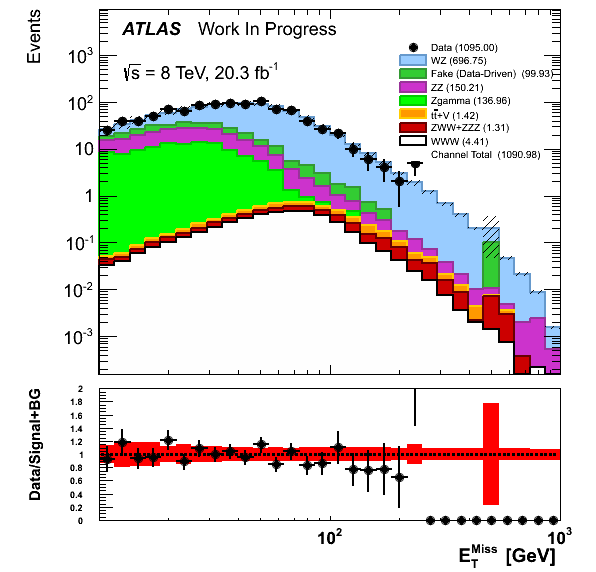
\includegraphics[width=0.4\columnwidth]{figures/appendix_signal_selection/Nov24Update_FakeSys_KFacSys_LogY_NoRebin/output/jobs/MxM/DataFull_Rates_May13_FakeRatesExactly2Loose_MuonMxMBJetGt0_ElBJetGt0SubtractPC_MxM/PreselectionNov23_15_1SFOS_ChargeAbs1_BVeto85_physics/weight_all/png/MET_Et_histratio.png}
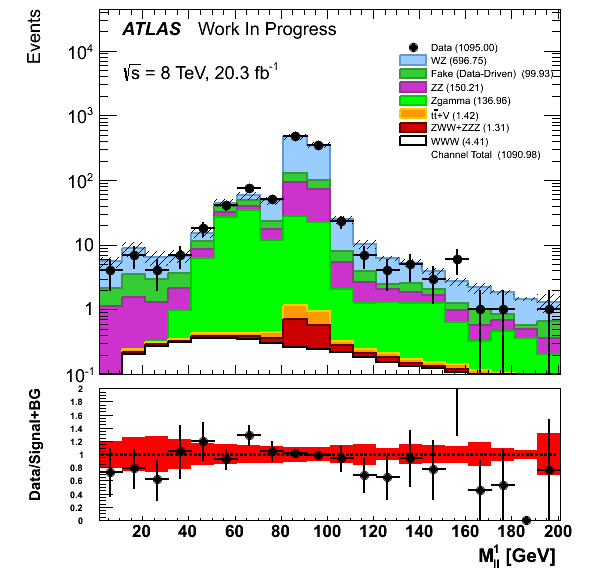
\includegraphics[width=0.4\columnwidth]{figures/appendix_signal_selection/Nov24Update_FakeSys_KFacSys_LogY_NoRebin/output/jobs/MxM/DataFull_Rates_May13_FakeRatesExactly2Loose_MuonMxMBJetGt0_ElBJetGt0SubtractPC_MxM/PreselectionNov23_15_1SFOS_ChargeAbs1_BVeto85_physics/weight_all/png/InvariantMassSFOS_histratio.png}
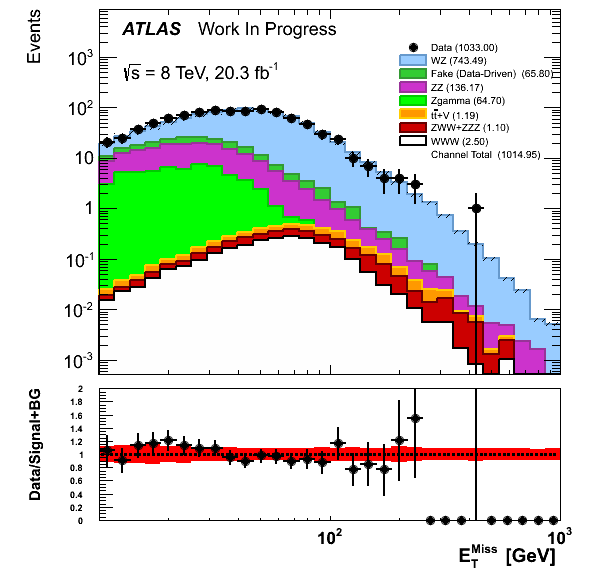
\includegraphics[width=0.4\columnwidth]{figures/appendix_signal_selection/Nov24Update_FakeSys_KFacSys_LogY_NoRebin/output/jobs/MxM/DataFull_Rates_May13_FakeRatesExactly2Loose_MuonMxMBJetGt0_ElBJetGt0SubtractPC_MxM/PreselectionNov23_15_2SFOS_ChargeAbs1_BVeto85_physics/weight_all/png/MET_Et_histratio.png}
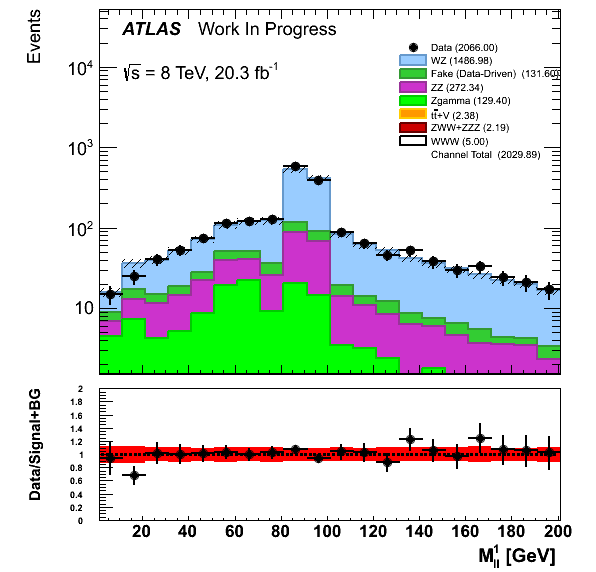
\includegraphics[width=0.4\columnwidth]{figures/appendix_signal_selection/Nov24Update_FakeSys_KFacSys_LogY_NoRebin/output/jobs/MxM/DataFull_Rates_May13_FakeRatesExactly2Loose_MuonMxMBJetGt0_ElBJetGt0SubtractPC_MxM/PreselectionNov23_15_2SFOS_ChargeAbs1_BVeto85_physics/weight_all/png/InvariantMassSFOS_histratio.png}
\caption{Plots of the \MET (left) and $m_{\textrm{SFOS}}$ (right) distributions 
in the 1 SFOS (top) and 2 SFOS (bottom) regions after pre-selection
plus the \bee-veto requirement.}
\label{fig:met_zwindow_optimization}
\end{figure}

The absence of any cut on the \MET~distribution in the 0 SFOS
region can be better understood by looking at the 
the efficiency for selection between 
the signal and the background as a function of the \MET~selection threshold.
This is shown in \fig\ref{fig:met_eff} both after pre-selection
and in the 0 SFOS region.
Clearly, the signal efficiency closely follows the background efficiency
in the 0 SFOS region. Thus, there is no change in the
signal-to-background ratio when cutting on the \MET~distribution
in the 0 SFOS region and thus no improvement in the sensitivity.
On the other hand, there are large shape differences 
between the signal
and background efficiencies at pre-selection, with the 
signal efficiency remaining flatter at low values of the \MET~
threshold. So, from this one would expect a selection
on the \MET~threshold to be useful in the 1 and 2 SFOS
regions which have a similar background composition. 
Indeed, this is what we observe.


\begin{figure}[ht!]
\centering
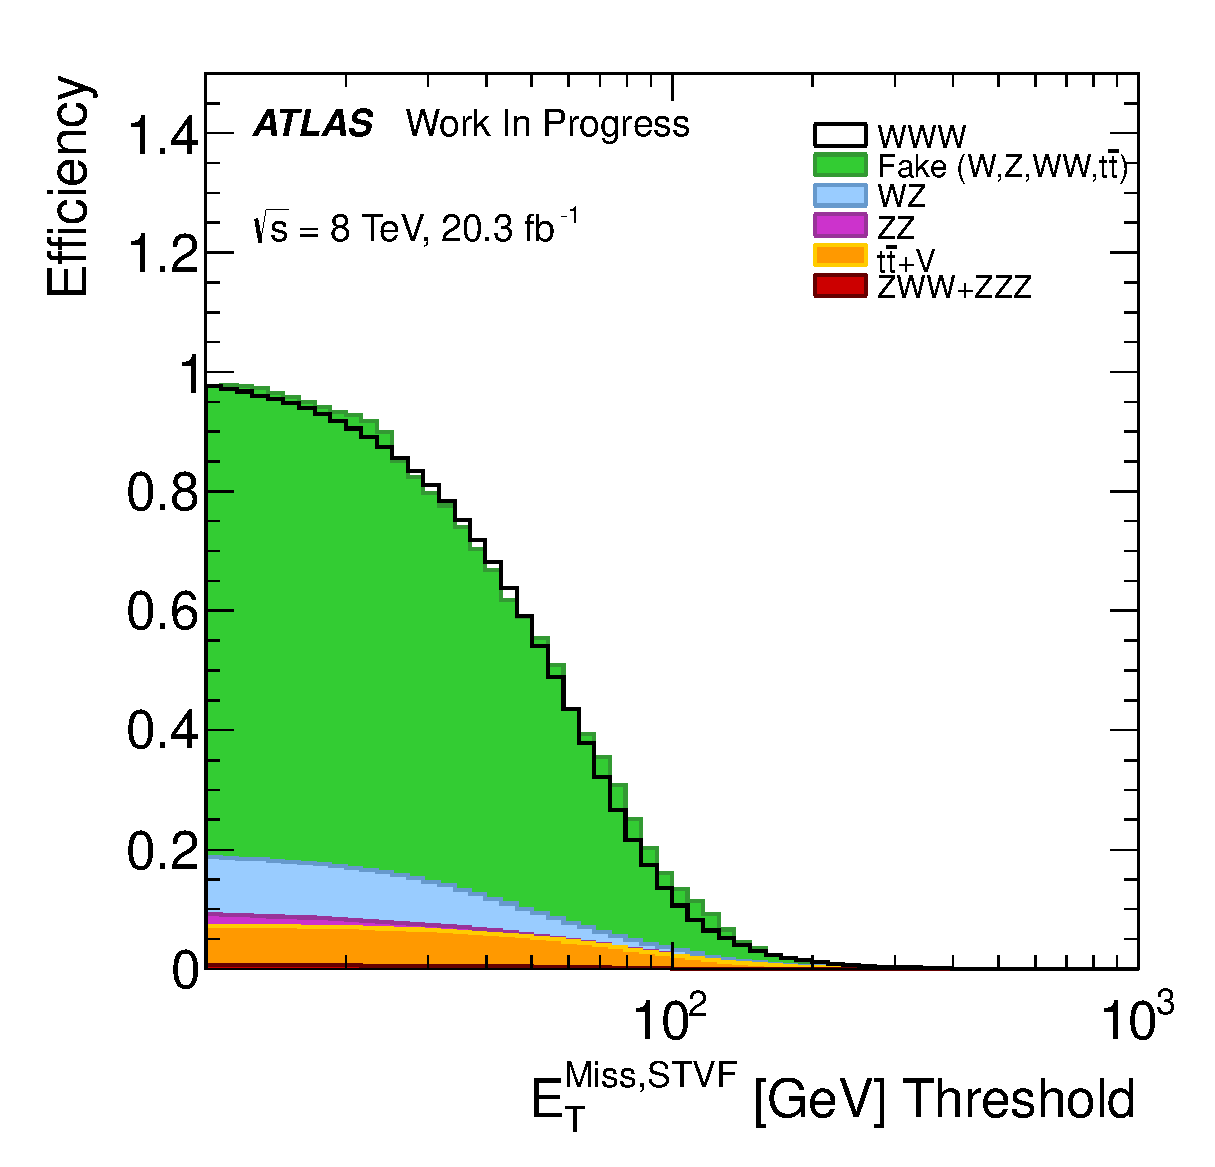
\includegraphics[width=0.45\columnwidth]{figures/optimization/SignalRegionsPreselection_0SFOS_Efficiencies/MET_Et_STVF_Cumulative.eps}
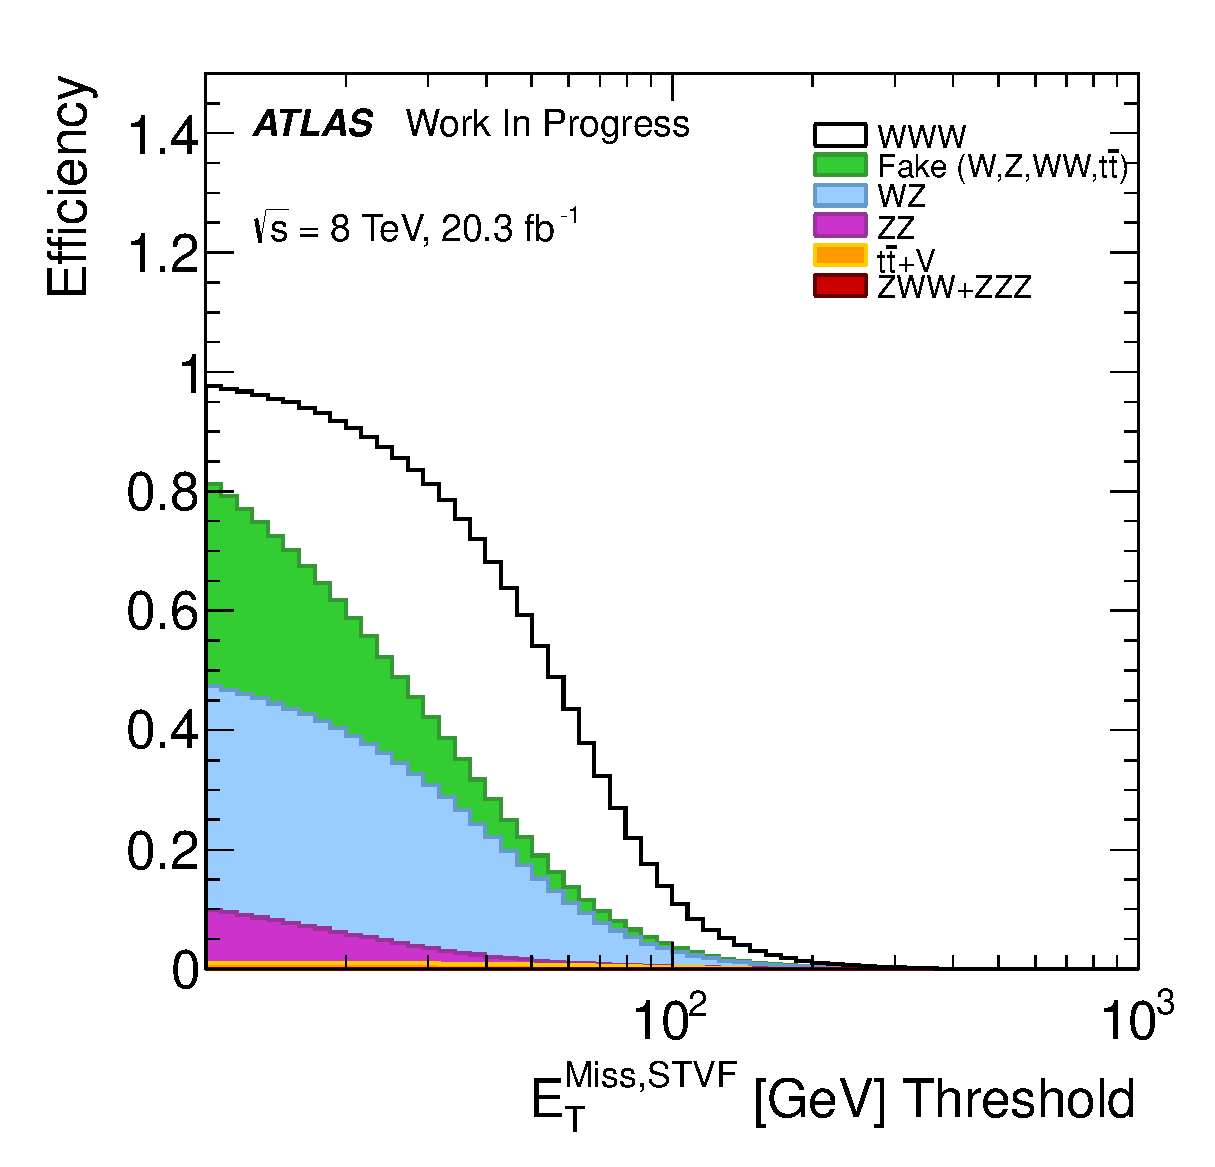
\includegraphics[width=0.45\columnwidth]{figures/optimization/SignalRegions_0p5mmZ0_Preselection_Efficiencies/MET_Et_STVF_Cumulative.eps}
\caption{ Signal and background efficiencies for the 
selection $\MET > X$ as a function of the \MET~selection
threshold, $X$,  in both the 0 SFOS (left) and pre-selection (right) regions.  }
\label{fig:met_eff}
\end{figure}

The threshold for the jet multiplicity cut 
of $\njet\leq 1$ applied in all signal regions
is also determined from the optimization. One might expect
that a different value for the threshold, such as a complete
veto on the presence of jets, would perform better. 
Indeed, looking at the efficiency for selection on the jet multiplicity
in \fig\ref{fig:njet_eff} does show a much stronger background
rejection when applying a veto in both the pre-selection region
and especially in the 0 SFOS region where there is a larger
contribution from fakes due to hadronic activity.
The signal rejection, however,  of about 40\% observed in both
regions, is prohibitive. Loosening the selection to the nominal
threshold of $\njet \leq 1$ instead preserves 90\% of the signal, 
which is quite precious.  We are still able to remove 
much of the fake background in the 0 SFOS region by vetoing
events with \bee-tagged jets as can be seen in \fig\ref{fig:nbjet_eff}.
%any mention of different operating points
It is possible that using a \bee-tagging operating point
with an even higher \bee-tagging efficiency would further 
improve the sensitivity in the 0 SFOS region.  
The nominal operating point used here, however,  is the highest 
efficiency operating point available.
Clearly, there is no advantage gained from using a looser operating point
as this would only cut less on the background without having an impact
on the signal.



\begin{figure}[ht!]
\centering
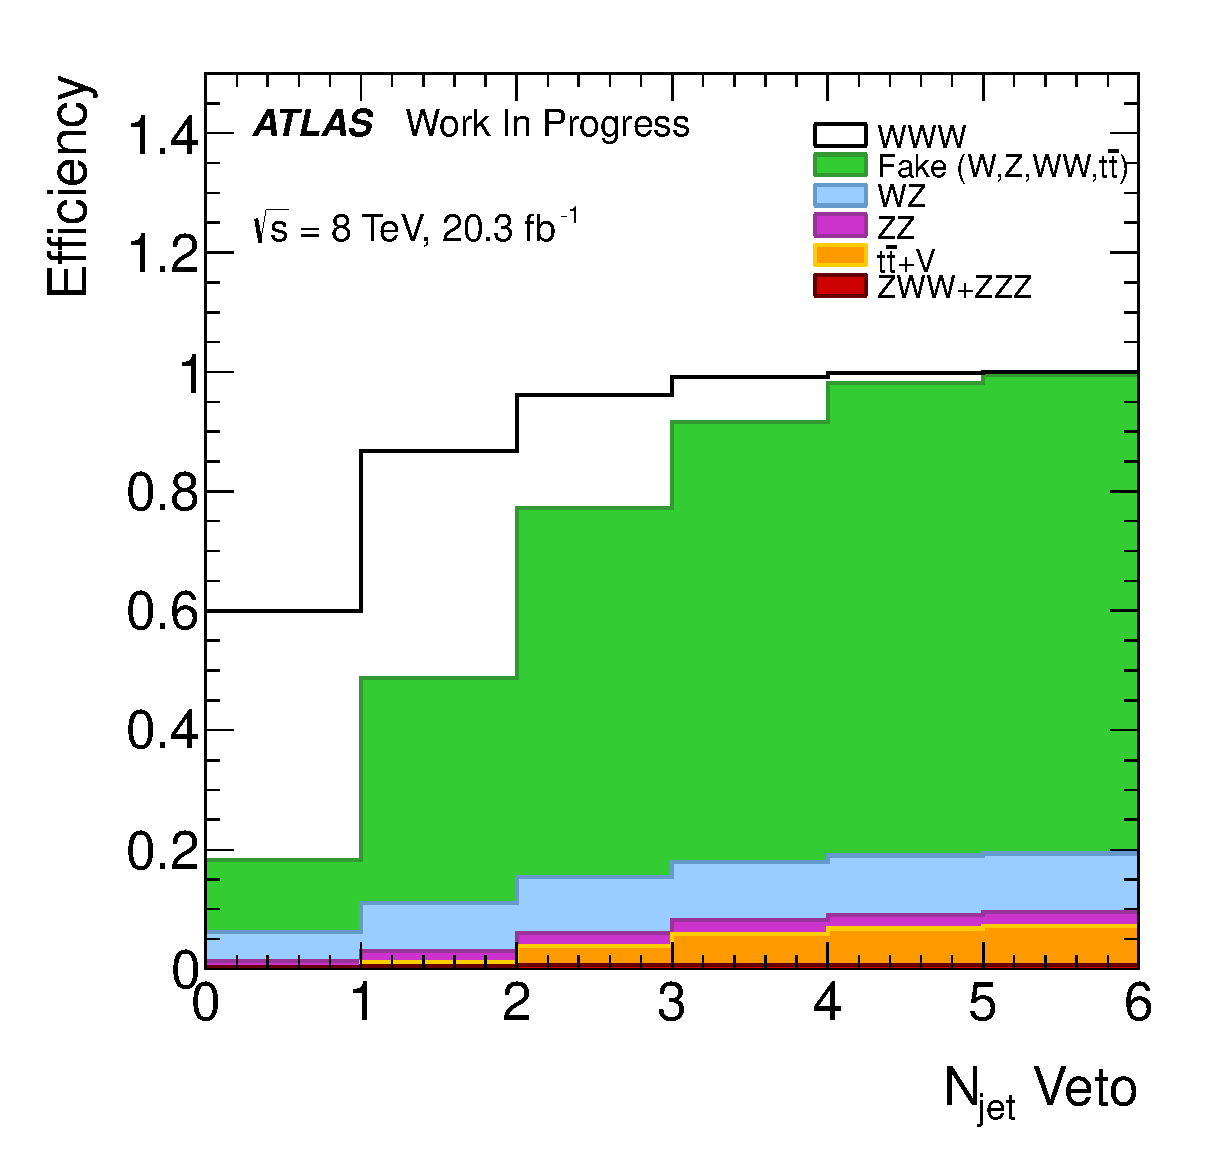
\includegraphics[width=0.45\columnwidth]{figures/optimization/SignalRegionsPreselection_0SFOS_Efficiencies/NJets_LeftCumulative.eps}
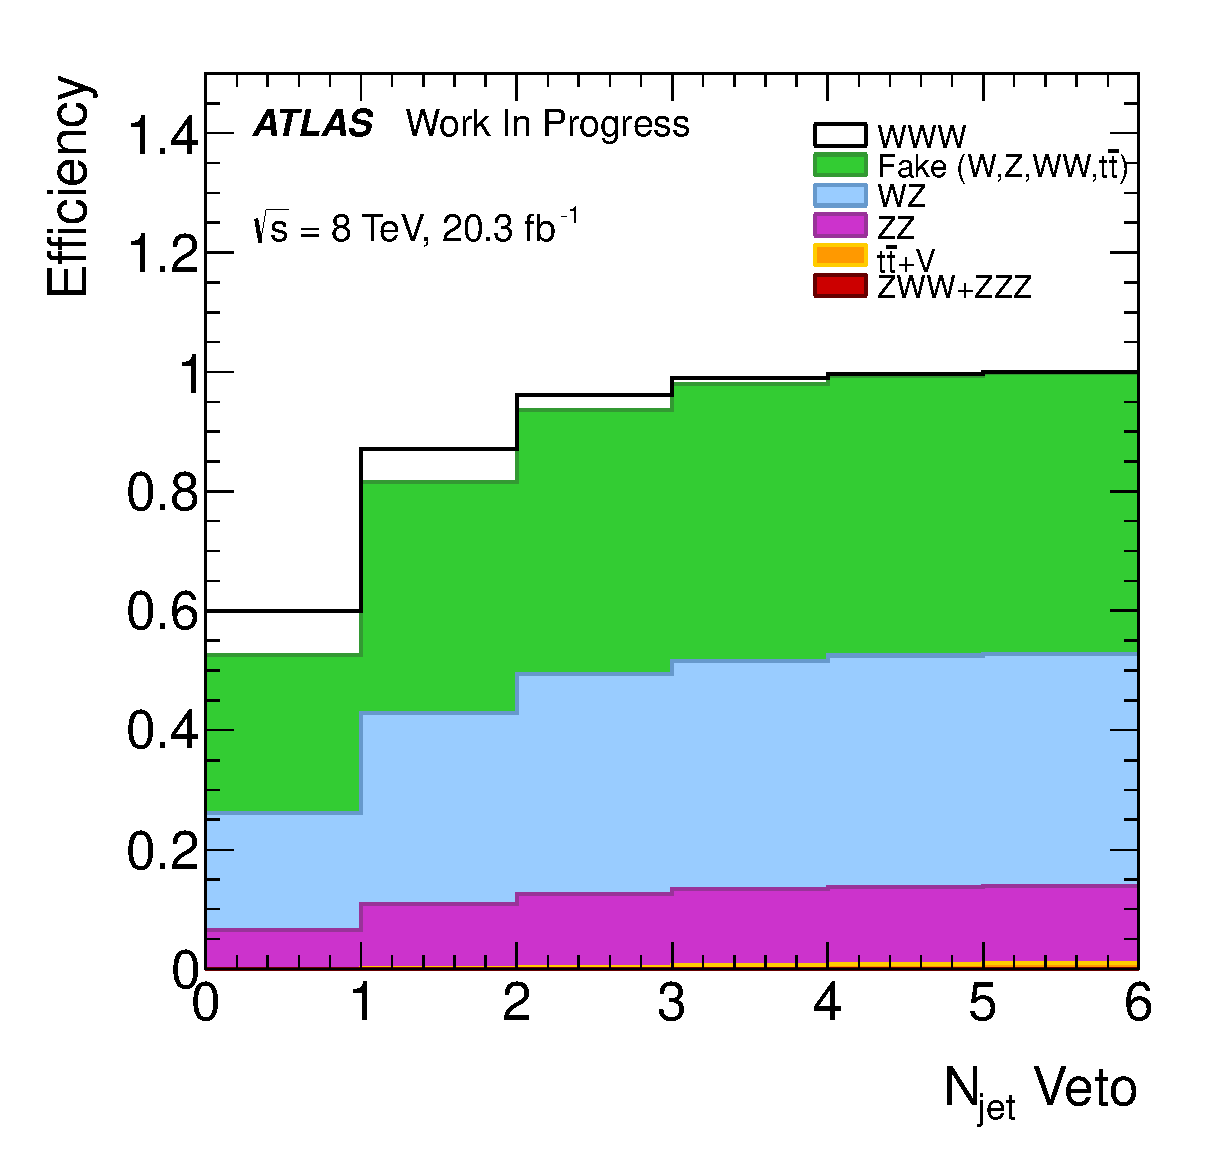
\includegraphics[width=0.45\columnwidth]{figures/optimization/SignalRegions_0p5mmZ0_Preselection_Efficiencies/NJets_LeftCumulative.eps}
\caption{ Signal and background efficiencies for the selection
$\njet \leq X$ as a function of the \njet~selection
threshold, $X$, in both the 0 SFOS (left) and pre-selection (right) regions.  }
\label{fig:njet_eff}
\end{figure}

\begin{figure}[ht!]
\centering
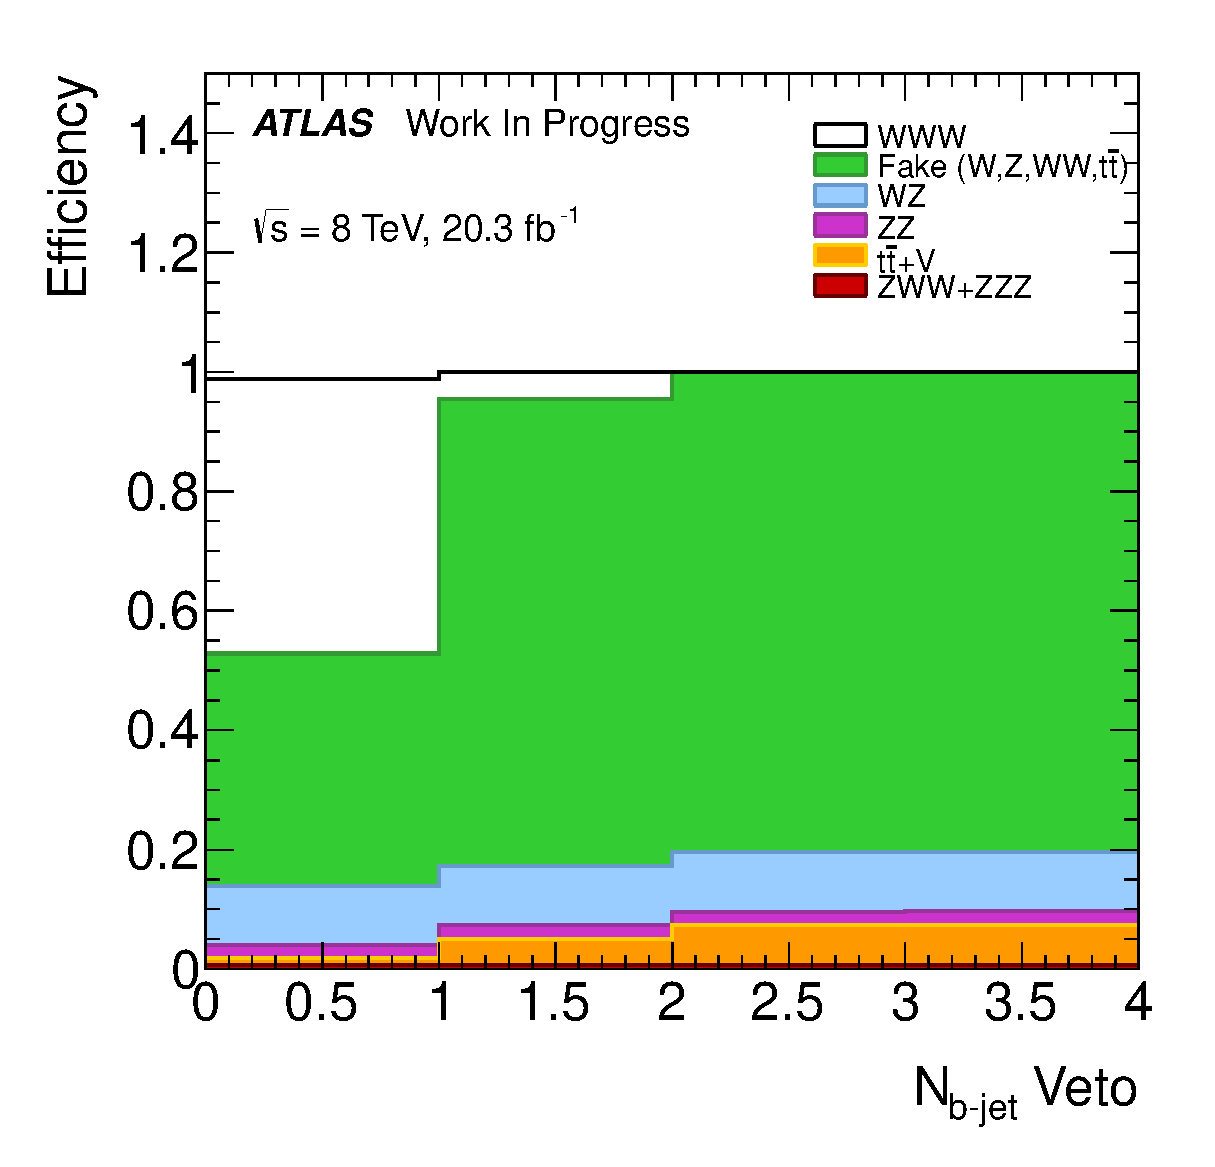
\includegraphics[width=0.45\columnwidth]{figures/optimization/SignalRegionsPreselection_0SFOS_Efficiencies/NBTaggedJets_LeftCumulative.eps}
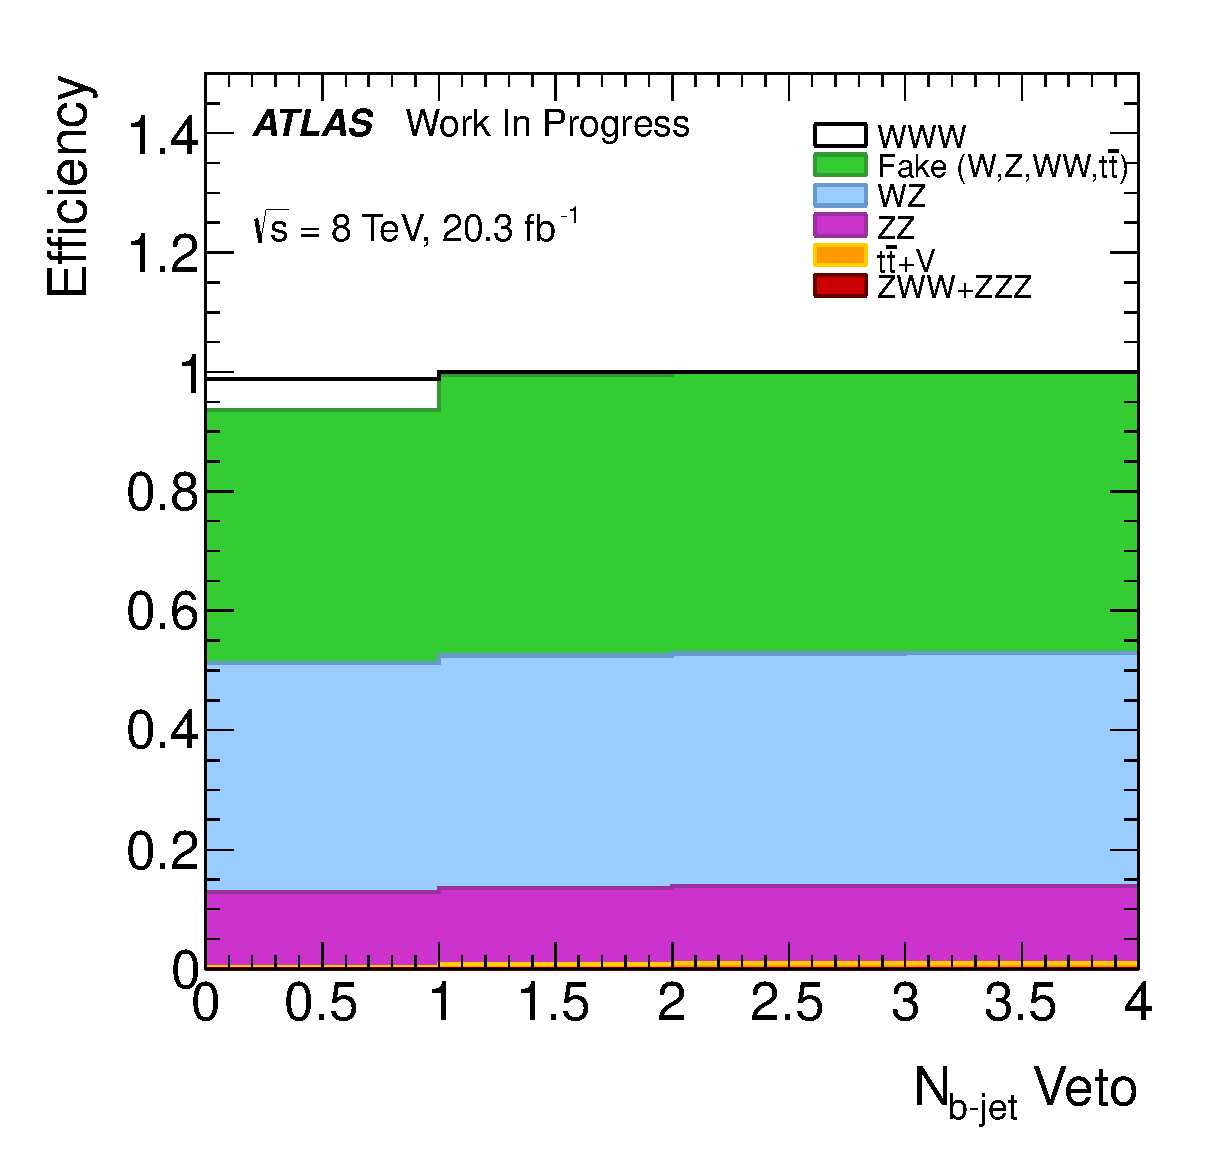
\includegraphics[width=0.45\columnwidth]{figures/optimization/SignalRegions_0p5mmZ0_Preselection_Efficiencies/NBTaggedJets_LeftCumulative.eps}
\caption{ Signal and background efficiencies 
for the selection
$\nbjet \leq X$
as a function of the \nbjet~selection
threshold, $X$, in both the 0 SFOS (left) and pre-selection (right) regions.  }
\label{fig:nbjet_eff}
\end{figure}


The \deltaphi~distribution for the signal is observed to be more back-to-back
(i.e. closer to $\pi$)
than that for the background. This is especially true in the 0 SFOS
region, as can be seen from the efficiencies plotted 
as a function of the \deltaphi~
selection threshold shown in \fig\ref{fig:deltaphi_eff}.
The selection efficiency for the signal is relatively flat for
most of the range up to about 
a threshold of $|\deltaphi|>2.5$ in both the pre-selection and 0 SFOS
regions.  At this threshold the signal selection efficiency 
is about 80\%.  The optimization prefers a selection
around this range for all signal regions.
The optimization also considered selecting on alternative
definitions of $\Delta\phi$ that only considered one of the three
leptons but this was observed to not offer as strong of a separation
between the signal and background. %figure?

\begin{figure}[ht!]
\centering
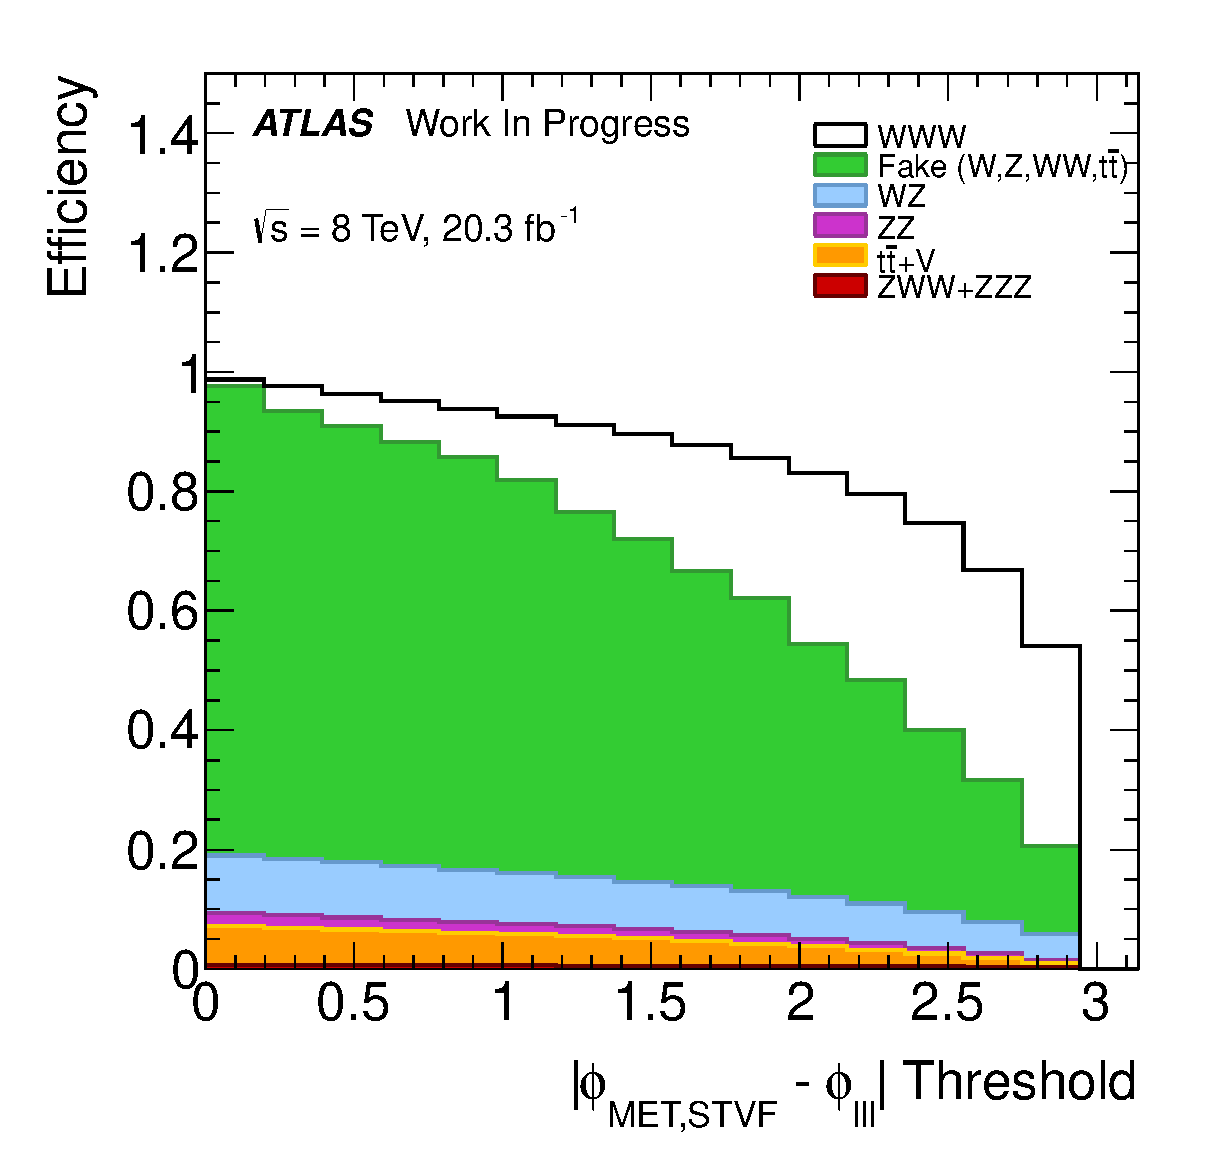
\includegraphics[width=0.45\columnwidth]{figures/optimization/SignalRegionsPreselection_0SFOS_Efficiencies/DeltaPhiMETSTVF123_Abs_Cumulative.eps}
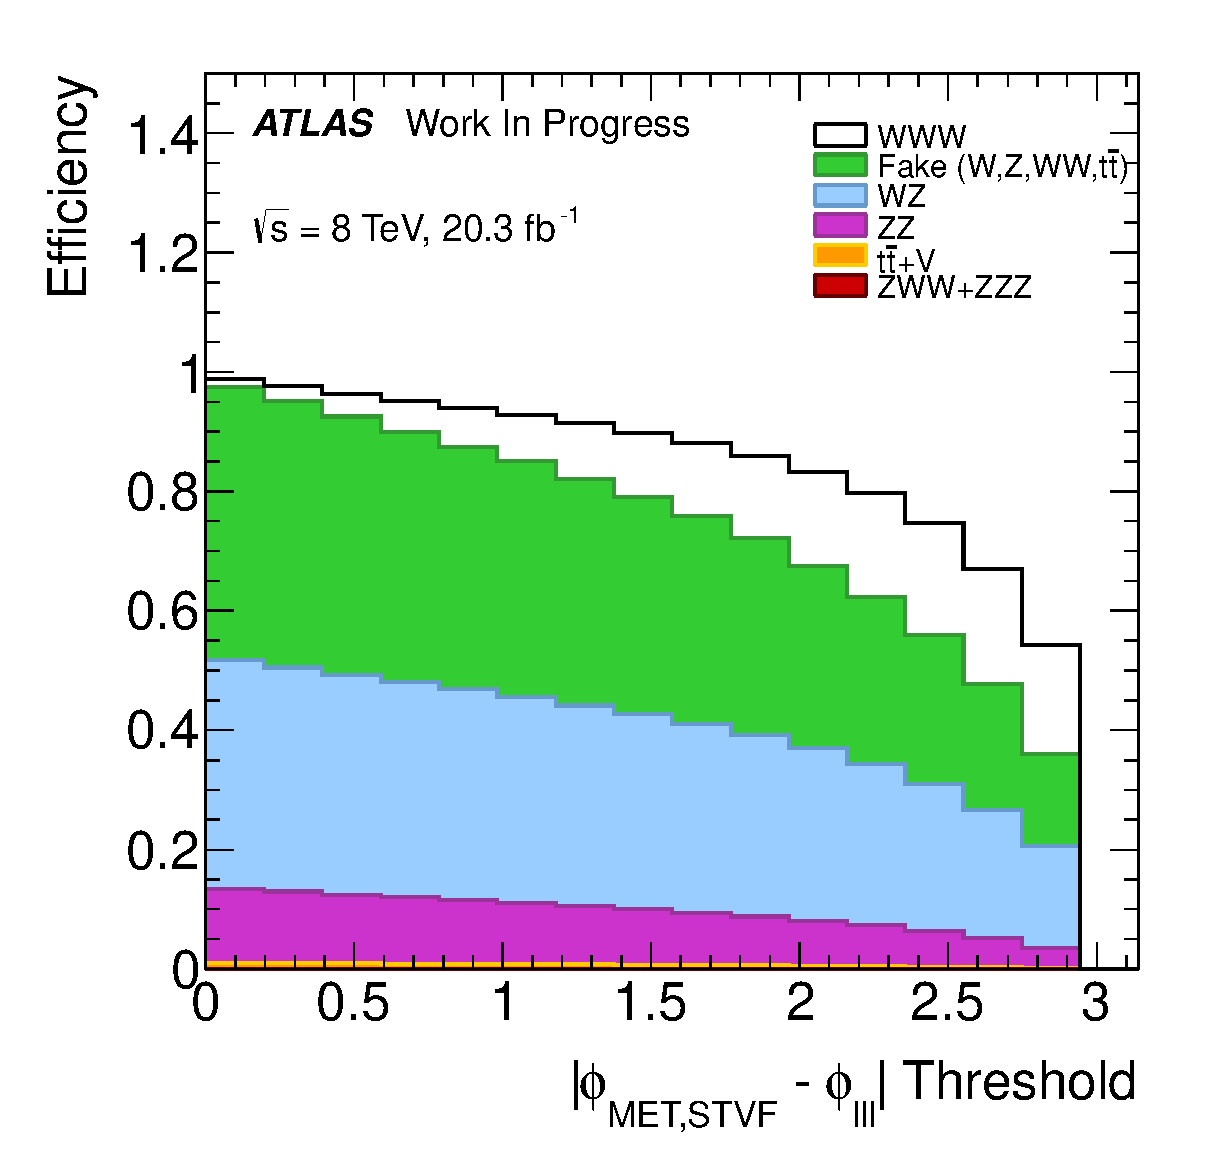
\includegraphics[width=0.45\columnwidth]{figures/optimization/SignalRegions_0p5mmZ0_Preselection_Efficiencies/DeltaPhiMETSTVF123_Abs_Cumulative.eps}
\caption{ Signal and background efficiencies 
for the selection
$|\deltaphi| > X$
as a function of the \deltaphi~selection
threshold, $X$, in both the 0 SFOS (left) and pre-selection (right) regions.  }
\label{fig:deltaphi_eff}
\end{figure}

The efficiencies as a function of the lepton \pt~threshold are shown 
in \fig\ref{fig:pt_eff}. 
The signal efficiency is observed to be slightly flatter
than the background efficiency.
The signal efficiency, however,  still falls fairly 
rapidly as a function of the lepton \pt~threshold. 
Thus, a tighter selection on the lepton \pt~is not preferred
by the optimization. We also considered 
applying different \pt~thresholds to the leptons
based on their \pt~order and other criteria, but
this did not show any increased performance.


\begin{figure}[ht!]
\centering
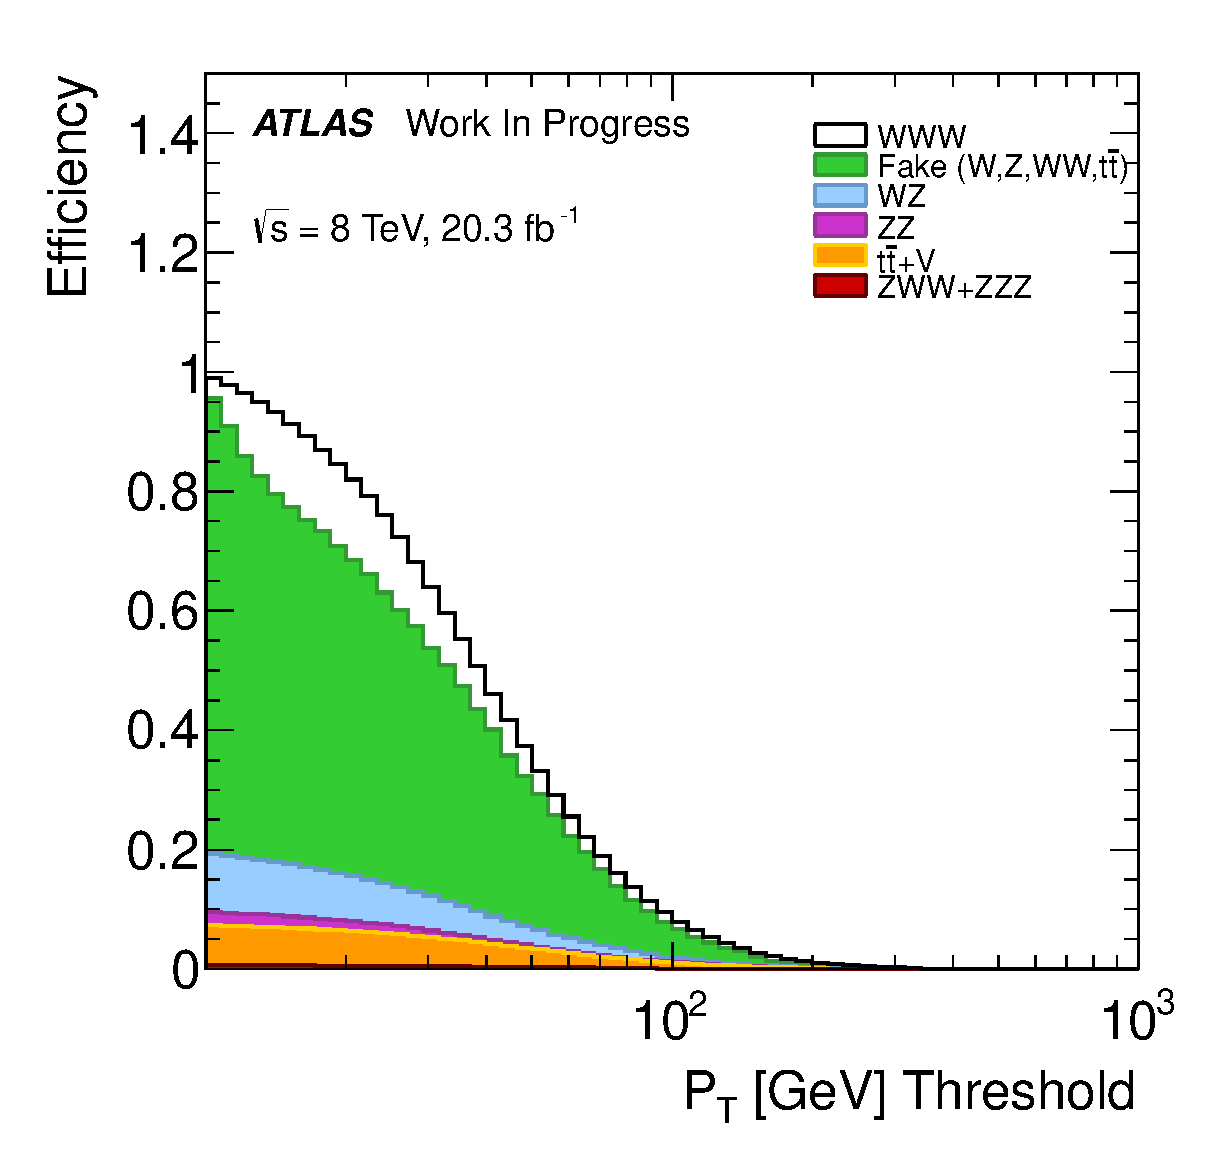
\includegraphics[width=0.45\columnwidth]{figures/optimization/SignalRegionsPreselection_0SFOS_Efficiencies/AllLeptonPt_Cumulative.eps}
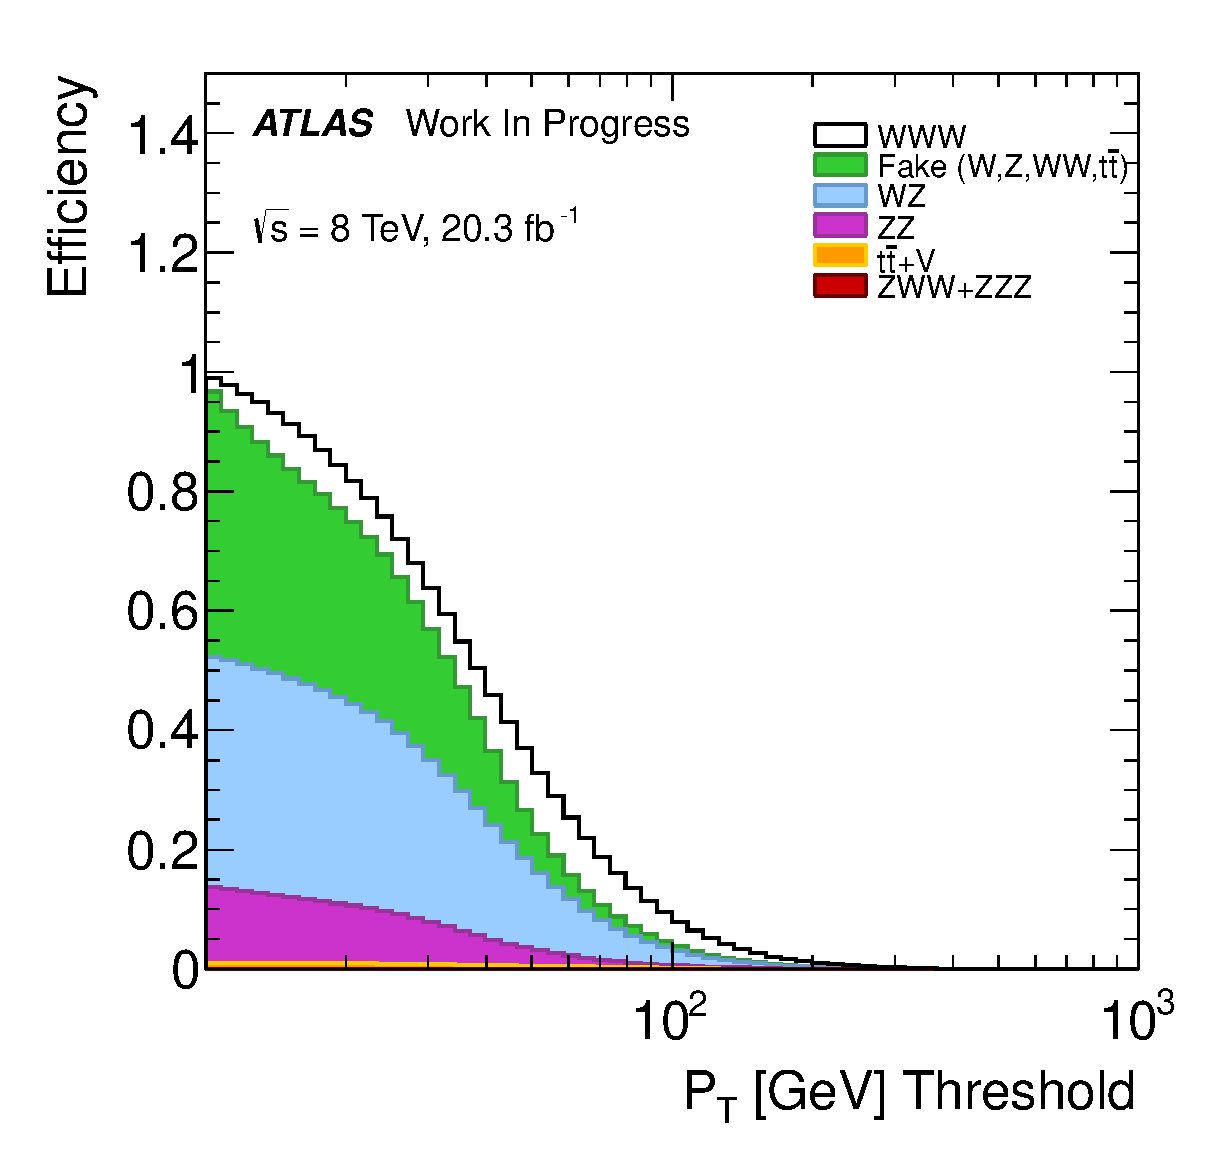
\includegraphics[width=0.45\columnwidth]{figures/optimization/SignalRegions_0p5mmZ0_Preselection_Efficiencies/AllLeptonPt_Cumulative.eps}
\caption{ Signal and background efficiencies 
for the selection
Lepton $\pt > X$
as a function of the \pt~selection
threshold, $X$, in both the 0 SFOS (left) and pre-selection (right) regions.  }
\label{fig:pt_eff}
\end{figure}

Finally, we considered other quantities like the 
transverse mass of the \MET~and three lepton system:
\begin{equation}
m_{T}^{lll} = \sqrt{2p_{T}^{lll}\MET(1-\cos(\Delta\varphi(lll,\MET)))}
\end{equation}
as well as vetoes on additional leptons with lower \pt, and various
di-lepton mass selections.  None of these, however, were preferred
by the optimization.


